\documentclass[12pt]{beamer}
\usepackage{../Estilos/BeamerMAF}
\usepackage[absolute, overlay]{textpos}
\usepackage{../Estilos/ColoresLatex}
\usetheme{Copenhagen}
\usecolortheme{wolverine}
%\useoutertheme{default}
\setbeamercovered{invisible}
% or whatever (possibly just delete it)
\setbeamertemplate{section in toc}[sections numbered]
\setbeamertemplate{subsection in toc}[subsections numbered]
\setbeamertemplate{subsection in toc}{\leavevmode\leftskip=3.2em\rlap{\hskip-2em\inserttocsectionnumber.\inserttocsubsectionnumber}\inserttocsubsection\par}
% \setbeamercolor{section in toc}{fg=blue}
% \setbeamercolor{subsection in toc}{fg=blue}
% \setbeamercolor{frametitle}{fg=blue}
\setbeamertemplate{caption}[numbered]

\setbeamertemplate{footline}
\beamertemplatenavigationsymbolsempty
\setbeamertemplate{headline}{}


\makeatletter
% \setbeamercolor{section in foot}{bg=gray!30, fg=black!90!orange}
% \setbeamercolor{subsection in foot}{bg=blue!30}
% \setbeamercolor{date in foot}{bg=black}
\setbeamertemplate{footline}
{
  \leavevmode%
  \hbox{%
  \begin{beamercolorbox}[wd=.333333\paperwidth,ht=2.25ex,dp=1ex,center]{section in foot}%
    \usebeamerfont{section in foot} \insertsection
  \end{beamercolorbox}%
  \begin{beamercolorbox}[wd=.333333\paperwidth,ht=2.25ex,dp=1ex,center]{subsection in foot}%
    \usebeamerfont{subsection in foot}  \insertsubsection
  \end{beamercolorbox}%
  \begin{beamercolorbox}[wd=.333333\paperwidth,ht=2.25ex,dp=1ex,right]{date in head/foot}%
    \usebeamerfont{date in head/foot} \insertshortdate{} \hspace*{2em}
    \insertframenumber{} / \inserttotalframenumber \hspace*{2ex} 
  \end{beamercolorbox}}%
  \vskip0pt%
}
\makeatother

\makeatletter
\patchcmd{\beamer@sectionintoc}{\vskip1.5em}{\vskip0.8em}{}{}
\makeatother

% %\newlength{\depthofsumsign}
% \setlength{\depthofsumsign}{\depthof{$\sum$}}
% \newcommand{\nsum}[1][1.4]{% only for \displaystyle
%     \mathop{%
%         \raisebox
%             {-#1\depthofsumsign+1\depthofsumsign}
%             {\scalebox
%                 {#1}
%                 {$\displaystyle\sum$}%
%             }
%     }
% }
% \def\scaleint#1{\vcenter{\hbox{\scaleto[3ex]{\displaystyle\int}{#1}}}}
% \def\scaleoint#1{\vcenter{\hbox{\scaleto[3ex]{\displaystyle\oint}{#1}}}}
% \def\bs{\mkern-12mu}


\setbeamercolor{section in foot}{bg=babyblue, fg=black}
\setbeamercolor{subsection in foot}{bg=blond, fg=black}


\makeatletter
\setbeamertemplate{footline}
{
\leavevmode%
\hbox{%
\begin{beamercolorbox}[wd=.333333\paperwidth,ht=2.25ex,dp=1ex,center]{section in foot}%
  \usebeamerfont{section in foot} \insertsection
\end{beamercolorbox}%
\begin{beamercolorbox}[wd=.333333\paperwidth,ht=2.25ex,dp=1ex,center]{subsection in foot}%
  \usebeamerfont{subsection in foot}  \insertsubsection
\end{beamercolorbox}%
\begin{beamercolorbox}[wd=.333333\paperwidth,ht=2.25ex,dp=1ex,right]{date in head/foot}%
  \usebeamerfont{date in head/foot} \insertshortdate{} \hspace*{1.5em}
  \insertframenumber{} / \inserttotalframenumber \hspace*{2ex} 
\end{beamercolorbox}}%
\vskip0pt%
}
\makeatother
\usefonttheme{serif}
\setbeamercolor{frametitle}{bg=champagne}
\resetcounteronoverlays{saveenumi}

\date{24 de mayo de 2022}

\title{\large{Oscilaciones en una membrana circular}}
\subtitle{Funciones de Bessel}
\author{M. en C. Gustavo Contreras Mayén}

\begin{document}
\maketitle
\fontsize{14}{14}\selectfont
\spanishdecimal{.}

\section*{Contenido}
\frame{\frametitle{Temas a revisar} \tableofcontents[currentsection, hideallsubsections]}

\section{Marco teórico}
\frame{\tableofcontents[currentsection, hideothersubsections]}
\subsection{Introducción}

\begin{frame}
\frametitle{Ondas estacionarias}
Consideramos ondas estacionarias en un sistema bidimensional con simetría circular: \pause la de una membrana circular delgada y flexible (por ejemplo, un parche circular de tambor idealizado) de radio $R$.
\end{frame}
\begin{frame}
\frametitle{Ecuación de onda}
La ecuación de onda en coordenadas cilíndricas en dos dimensiones $(x , y \to r, \varphi)$ para la amplitud del desplazamiento, $\psi (r, \varphi, t)$ viene dada por:
\pause
\begin{align*}
\laplacian{\psi} (r, \varphi, t) - \dfrac{1}{v^{2}} \, \pdv[2]{\psi (r, \varphi, t)}{t} = 0
\end{align*}
\end{frame}
\begin{frame}
\frametitle{Velocidad longitudinal}
Donde la velocidad longitudinal de propagación de ondas transversales en una membrana circular bidimensional estirada está (también) dada por:
\pause
\begin{align*}
v = \sqrt{\dfrac{T_{\ell}}{\sigma}}
\end{align*}
\end{frame}
\begin{frame}
\frametitle{Velocidad longitudinal}
\begin{align*}
v = \sqrt{\dfrac{T_{\ell}}{\sigma}}
\end{align*}
donde:
\setbeamercolor{item projected}{bg=yellow,fg=black}
\setbeamertemplate{enumerate items}{%
\usebeamercolor[bg]{item projected}%
\raisebox{1.5pt}{\colorbox{bg}{\color{fg}\footnotesize\insertenumlabel}}%
}
\begin{enumerate}[<+->]
\item $T_{\ell}$ es la tensión superficial de la membrana (en $\si{\newton\per\metre}$).
\item $\sigma \equiv M/A = M / \pi \, R^{2}$ es la densidad de masa superficial de la membrana (en $\si{\kilo\gram\per\square\metre}$).
\end{enumerate}
\end{frame}
\begin{frame}
\frametitle{Laplaciano en coord. cilíndricas}
Con $x = r \, \cos \varphi$, $y = r \, \sin \varphi$, $\dd[2]{r} = r \, \dd{r} \dd{\varphi}$, \pause el operador Laplaciano, $\laplacian$ en coordenadas cilíndricas en 2D viene dado por:
\pause
\begin{align*}
\laplacian = \dfrac{1}{r} \, \pdv{r} \left( r \, \pdv{r} \right) + \dfrac{1}{r^{2}} \, \pdv[2]{\phi}
\end{align*}
\end{frame}
\begin{frame}
\frametitle{Ec. de onda en 2D cilíndricas}
Así, la ecuación de onda bidimensional que describe el comportamiento de las ondas en una membrana cilíndrica viene dada por:
\pause
\begin{align*}
\pdv[2]{\psi}{r} + \dfrac{1}{r} \pdv{\psi}{r} + \dfrac{1}{r^{2}} \, \pdv[2]{\psi}{\varphi} = \dfrac{1}{v^{2}} \, \pdv[2]{\psi}{t}
\end{align*}
\end{frame}
\begin{frame}
\frametitle{Observaciones}
Notemos que el lado izquierdo de la igualdad (lado derecho de la igualdad) contiene solo funciones dependientes del espacio (dependientes del tiempo), respectivamente.
\end{frame}

\section{Separación de variables}
\frame{\tableofcontents[currentsection, hideothersubsections]}
\subsection{Solución propuesta}

\begin{frame}
\frametitle{Usando separación de variables}
Por lo tanto, podemos usar la técnica de separación de variables, con:
\pause
\begin{align*}
\psi (r, \varphi, t) = U(r, \varphi) \, T(t)
\end{align*}
\pause
donde $U (r, \varphi)$ contiene solo términos espacialmente dependientes de $r$ y $\varphi$ y $T (t)$ contiene solo el término dependiente del tiempo.
\end{frame}
\begin{frame}
\frametitle{Relación de la velocidad}
Tenemos la relación
\begin{eqnarray*}
\begin{aligned}
v &= f \lambda = \\[0.5em] \pause
&=  \left( \dfrac{\omega}{2 \, \pi} \right) \left( \dfrac{2 \, \pi}{k} \right) = \\[0.5em] \pause
&= \dfrac{\omega}{k}
\end{aligned}
\end{eqnarray*}
\pause
entonces $v \, k = \omega$.
\end{frame}
\begin{frame}
\frametitle{Primera constante de separación}
Obtenemos una constante de separación $-k^{2}$, \pause y después de realizar algunas manipulaciones algebraicas simples, llegamos a las siguientes ED2H:
\pause
\begin{eqnarray*}
\begin{aligned}
\pdv[2]{\psi}{r} + \dfrac{1}{r} \pdv{\psi}{r} + \dfrac{1}{r^{2}} \, \pdv[2]{\psi}{\varphi} + k^{2} \, U(r, \varphi) &= 0\\[0.5em]
\dv[2]{T(t)}{t} + \omega \, T(t) &= 0
\end{aligned}
\end{eqnarray*}
\end{frame}
\begin{frame}
\frametitle{Separando nuevamente la ecuación}
Podemos usar nuevamente la técnica de separación de variables en la ecuación espacial anterior, \pause con una solución de producto de la forma:
\pause
\begin{align*}
U(r, \varphi) = R(r) \, \Phi (\varphi)
\end{align*}
\end{frame}
\begin{frame}
\frametitle{Juntando los resultados}
Incorporando este producto en la ecuación espacial anterior y realizando las diferenciaciones (parciales), \pause dividiendo por $U(r, \varphi)$ y realizando una manipulación algebraica simple, \pause obtenemos la siguiente ecuación:
\pause
\begin{align*}
\dfrac{1}{R} \left( r^{2} \, \dv[2]{R}{r} +  r \, \dv{R}{r} + k^{2} \, r^{2} \, R(r) \right) = - \dfrac{1}{\Phi} \, \dv[2]{\Phi}{\varphi}
\end{align*}
\end{frame}
\begin{frame}
\frametitle{Resultado de la separación}
El lado izquierdo de la igualdad (el lado derecho) de esta ecuación depende solo de $r$ (solo de $\varphi$), respectivamente.
\\
\bigskip
\pause
Nuevamente, esto solo puede ser cierto para todos los valores posibles de $(r, \varphi)$, si tanto el lado izquierdo de la expresión como el lado derecho, son iguales a una constante (adimensional).
\end{frame}

\subsection{Soluciones periódicas}

\begin{frame}
\frametitle{Soluciones periódicas}
Sabemos que las soluciones $\Phi(\varphi)$ deben ser periódicas y univaluadas, es decir:
\pause 
\begin{align*}
\Phi (\varphi = 0) = \Phi (\varphi = 2 \, \pi)
\end{align*}
\end{frame}
\begin{frame}
\frametitle{Soluciones periódicas}
De manera general:
\pause
\begin{align*}
\Phi (\varphi = \varphi_{0}) &= \Phi (\varphi = \varphi_{0} + 2 \, m \, \pi), \\[0.em]
&m = 0, \pm 1, \pm 2,\pm 3, \ldots
\end{align*}
\pause
Por lo tanto, elegiremos esta constante de separación para que sea $m^{2}$.
\end{frame}
\begin{frame}
\frametitle{Las eigenfunciones}
Las eigenfunciones de $\Phi_{m} (\varphi)$ son (una de) las dos siguientes formas equivalentes:
\pause 
\begin{align*}
\Phi_{m} (\varphi) &= \alpha_{m} \, \cos m \, \varphi + \beta \, \sin m \, \varphi \\[1em]
&\begin{cases}
-1 \leq \alpha_{m} \leq 1, \\
-1 \leq \beta_{m} \leq 1 \\
\sqrt{\alpha_{m}^{2} + \beta_{m}^{2}} = 1
\end{cases}
\end{align*}
\end{frame}
\begin{frame}
\frametitle{Las eigenfunciones}
La segunda forma es:
\pause
\begin{align*}
\Phi_{m} (\varphi) &= \exp(i (m \, \varphi + \delta_{m})) \hspace{0.6cm} \delta_{m} = \tan^{-1} \left( \dfrac{\beta_{m}}{\alpha_{m}}\right) \\[1em]
&\mbox{con } m = 0, \pm 1, \pm 2, \ldots
\end{align*}
\end{frame}

\subsection{Ecuación de Bessel}

\begin{frame}
\frametitle{Ecuación de Bessel}
La ecuación radial es la conocida ecuación diferencial de Bessel:
\pause
\begin{align*}
\dv[2]{R}{r} + \dfrac{1}{r} \, \dv{R}{r} + \left( k^{2} - \dfrac{m^{2}}{r^{2}} \right) \, R = 0
\end{align*}
\end{frame}
\begin{frame}
\frametitle{Solución a la Ec. de Bessel}
La solución más general a la ecuación de Bessel, con $m$ entero (que es el caso que aquí tenemos), es de la forma:
\pause
\begin{align*}
R_{m} (r) = A_{m} \, J_{m} (k \, r) + B_{m} \, Y_{m} (k \, r)
\end{align*}
donde $J_{m} (x)$ son las funciones ordinarias de Bessel de orden $m$, y las $Y_{m} (x)$ son las funciones de Bessel de segundo orden.
\end{frame}
\begin{frame}
\frametitle{Característica de las $J_{m} (x)$}
Las funciones $J_{m} (x)$ son finitas en $x = 0$ y se expresan normalmente en términos de una serie de potencias en $x$:
\pause
\begin{align*}
J_{m} (x) = \sum_{r=0}^{\infty} \dfrac{(-1)^{r}}{r! \, \Gamma(m + r + 1)} \, \left( \dfrac{x}{2} \right)^{m+2r}
\end{align*}
\end{frame}
\begin{frame}
\frametitle{Funciones para $m$ entero}
Sabemos que para $m$ entero: $J_{-m}(x) = (-1)^{m} \, J_{m}(x)$.
\\
\bigskip
\pause
Las funciones $Y_{m}(x)$ se pueden expresar de diversas maneras, entre ellas:
\pause
\begin{align*}
Y_{m}(x) = \dfrac{J_{m}(x) \, \cos (m \, \pi) - J_{-m}(x)}{\sin (m \, \pi)}
\end{align*}
\end{frame}
\begin{frame}
\frametitle{Funciones para $m$ entero}
Para $m$ entero, también se pueden escribir como:
\pause
\begin{align*}
Y_{m}(x) = \dfrac{1}{\pi} \left[ \pdv{J_{m}(x)}{m} - (-1)^{m} \, \pdv{J_{-m}(x)}{m} \right]
\end{align*}
\end{frame}
\begin{frame}
\frametitle{Las funciones de segunda clase}
Las funciones $Y_{m} (x)$ son singulares (se vuelven (negativas) infinitas) en $x = 0$.
\\
\bigskip
\pause
Sin embargo, debido a que usamos coordenadas cilíndricas para nuestra membrana circular, el origen $(r = 0)$ \textbf{se incluye} en este problema.
\end{frame}
\begin{frame}
\frametitle{Criterio importante}
Físicamente, \textbf{NO} se permiten desplazamientos de amplitud infinitos tal que $R(r) \to \infty$ para cualquier valor de $r$, ya que una suposición inicial implícita eran oscilaciones de \emph{amplitud pequeñas}. 
\end{frame}
\begin{frame}
\frametitle{Criterio importante}
Por tanto, todos los coeficientes $B_{m}$ para el $Y_{m} (x)$ deben ser $B_{m} = 0$ para soluciones en valores propios físicamente permitidas de la membrana circular bidimensional.
\end{frame}
\begin{frame}
\frametitle{Condición de frontera}
La condición de frontera radial para ondas estacionarias transversales en una membrana circular con borde fijo (es decir, desplazamiento transversal cero) en $r = R$ es $R_{m} (r = R) = 0$, \pause es decir, $J_{m} (k \, R) = 0$.
\end{frame}
\begin{frame}
\frametitle{Las raíces de $J_{m}(x)$}
Dado que $r = R > 0$, esto significa que buscamos los ceros de $J_{m} (k \, R)$, es decir, $J_{m} (x = k \,R) = 0$.
\\
\bigskip
\pause
Debido a la complejidad de la forma de $J_{m} (x)$, los ceros de $J_{m} (x)$ (y $Y_{m} (x)$) son de naturaleza no analítica, más bien, están tabulados en muchos libros de matemáticas, o pueden determinarse mediante técnicas numéricas gráficas y/o computacionales.
\end{frame}
\begin{frame}
\frametitle{Algunas raíces}
Presentamos los primeros ceros del $J_{m} (x)$ de orden inferior en la siguiente tabla:
\fontsize{12}{12}\selectfont
\begin{table}[H]
\centering
\begin{tabular}{c c c c c c}
    & & & $n=1$ & $n=2$ & $n=3$ \\
$m=0:$ & $J_{0}(x)=0:$ & $x \approx$ & $2.40$ & $5.52$ & $8.65  \ldots$ \\
$m=1:$ & $J_{1}(x)=0:$ & $x \approx$ & $3.83$ & $7.02$ & $10.17 \ldots$ \\
$m=2:$ & $J_{2}(x)=0:$ & $x \approx$ & $5.14$ & $8.42$ & $11.62 \ldots$ \\
\vdots
\end{tabular}
\end{table}
\end{frame}
\begin{frame}
\frametitle{Manejando dos índices}
Dado que $x = k \, R$, entonces $k = x / R$ y observando nuevamente, para este problema de eigenvalores de onda estacionaria bidimensional, \textbf{tenemos dos índices}: $m$ y $n$ para denotar:
\end{frame}
\begin{frame}
\frametitle{Manejando dos índices}
\setbeamercolor{item projected}{bg=yellow,fg=black}
\setbeamertemplate{enumerate items}{%
\usebeamercolor[bg]{item projected}%
\raisebox{1.5pt}{\colorbox{bg}{\color{fg}\footnotesize\insertenumlabel}}%
}
\begin{enumerate}[<+->]
\item Los eigenvalores de onda $k_{m, n}= x_{m, n} / R$,
\item Las eigenfrecuencias $\omega_{m, n}  = v \, k_{m, n}$  $f_{m, n} = v / \lambda_{m, n}$ con $v = \sqrt{T_{\ell} / \sigma}$,
\item Las eigenenergías, $E_{m, n} = \dfrac{1}{4} M \, \omega_{m, n}^{2} \, A_{m, n}^{2}$
\item Las eigenfunciones $\psi_{m, n} (r, \varphi, t) = R_{m,n} (r, \varphi, t) \, \Phi_{m} (\varphi) \, T_{m, n} (t)$
\end{enumerate}
\end{frame}
\begin{frame}
\frametitle{Soluciones ecuación temporal}
Las soluciones en eigenmodos de la ecuación de onda temporal asociada para ondas estacionarias bidimensionales en una membrana circular son de la siguiente(s) forma(s) equivalente(s):
\pause
\begin{align*}
\mathbf{i)} \hspace{0.15cm} T_{m,n} (t) &= b_{m,n} \, \sin (\omega_{m,n} \, t) {+} c_{m,n} \, \cos (\omega_{m,n} \, t) \\[0.5em]
-1 &\leq b_{m,n} \leq 1 \hspace{1cm} -1 \leq c_{m,n} \leq 1 \\[0.5em]
&\sqrt{b_{m,n}^{2} + c_{m,n}^{2}} = 1 \\[0.5em]
\end{align*}
\end{frame}
\begin{frame}
\frametitle{Soluciones ecuación temporal}
\begin{eqnarray*}
\begin{aligned}
\mathbf{ii)} \hspace{0.2cm} T_{m,n} (t) &= \sin (\omega_{m,n} \, t + \delta_{m,n}) = \\[0.5em] \pause
&= \cos(\omega_{m,n} \, t + \varphi_{m,n}) \\[0.5em] \pause
\delta_{m,n} = \varphi_{m,n} &+ \dfrac{\pi}{2} \\[0.5em] \pause
\mathbf{ii)} \hspace{0.2cm} T_{m,n} (t) &= \exp(i(\omega_{m,m} \, t + \varphi_{m,n}))
\end{aligned}
\end{eqnarray*}
\end{frame}

\section{Solución completa}
\frame{\tableofcontents[currentsection, hideothersubsections]}
\subsection{Eigenmodos}

\begin{frame}
\frametitle{Solución completa}
Las soluciones completas en eigenmodos para ondas estacionarias bidimensionales en una membrana circular de radio, $R$ con bordes fijos están dadas por alguna de las siguientes expresiones que son equivalentes:
\end{frame}
\begin{frame}
\frametitle{Solución completa}
\begin{eqnarray*}
\begin{aligned}
&\psi_{m,n} (r ,\varphi, t) = R_{m,n} (r) \, \Phi_{m} (\varphi) \, T_{m,n} (t) \\[0.5em] \pause
&\psi_{m,n} (r ,\varphi, t) = A_{m,n} \, J_{m,n} (k_{m,n} \, R) \times \\[0.5em]
&\times \exp(i(m \, \varphi + \delta_{m,n})) \, \exp(i(\omega_{m,n} \, t + \varphi_{m,n}))
\end{aligned}
\end{eqnarray*}
\end{frame}
\begin{frame}
\frametitle{Solución completa}
\begin{align*}
\psi_{m,n} (r ,\varphi, t) &= A_{m,n} \, J_{m,n} (k_{m,n} \, R) \times \\[0.5em]
&\times \big[ \alpha_{m,n} \,  \cos (m \, \varphi) + \beta_{m} \, \sin (m \, \varphi) \big] \times \\[0.5em]
&\times \big[ b_{m,n} \,  \cos (\omega_{m,n} \, t) + c_{m,n} \, \sin (\omega_{m,n} \, t) \big]
\end{align*}   
\end{frame}
\begin{frame}
\frametitle{Elementos propios}
Con:
\setbeamercolor{item projected}{bg=yellow,fg=black}
\setbeamertemplate{enumerate items}{%
\usebeamercolor[bg]{item projected}%
\raisebox{1.5pt}{\colorbox{bg}{\color{fg}\footnotesize\insertenumlabel}}%
}
\begin{enumerate}[<+->]
\item Eigenfrecuencias:
\begin{eqnarray*}
f_{m,n} = \dfrac{\omega_{m,n}}{2 \, \pi} = \pause \dfrac{v \, k_{m,n}}{2 \, \pi} = \pause \dfrac{v}{\lambda_{m,n}}
\end{eqnarray*}
\item Longitudes de onda propias:
\begin{eqnarray*}
\lambda_{m,n} = \dfrac{2 \, \pi}{k_{m,n}} = \pause \dfrac{2 \, \pi \, R}{x_{m,n}}
\end{eqnarray*}
\seti
\end{enumerate}
\end{frame}
\begin{frame}
\frametitle{Elementos propios}
\setbeamercolor{item projected}{bg=yellow,fg=black}
\setbeamertemplate{enumerate items}{%
\usebeamercolor[bg]{item projected}%
\raisebox{1.5pt}{\colorbox{bg}{\color{fg}\footnotesize\insertenumlabel}}%
}
\begin{enumerate}[<+->]
\conti    
\item Eigenenergías:
\begin{align*}
E_{m,n} = \dfrac{1}{4} \, M \, \omega_{m,n}^{2} \, A_{m,n}^{2}
\end{align*}
\begin{align*}
m = 0, 1, 2, 3, \ldots \hspace{1cm} n = 1, 2, 3, \ldots
\end{align*}
\end{enumerate}
\end{frame}

\subsection{Modos de vibración}

\begin{frame}
\frametitle{Modos bajos de vibración}
Los modos más bajos de ondas estacionarias transversales en una membrana circular se enumeran a continuación:
\end{frame}
\begin{frame}
\frametitle{Modos bajos de vibración}
\fontsize{10}{10}\selectfont
\begin{table}[H]
\centering
\begin{tabular}{c c c c l}
$m {=} 0$ & $n {=} 1$ & $k_{0,1} {\approx} 2.40/R$ & $\omega_{0,1} {\approx} 2.40 \, v/R$ & \\[0.5em] 
\multicolumn{5}{l}{$\psi_{0,1}(r, \varphi, t) {=} A_{0,1} \, J_{0}(k_{0,1} \, R) \, T_{0,1}(t)$} \\[0.5em] \hline \pause
$m {=} 1$ & $n {=} 1$ & $k_{1,1} {\approx} 3.83/R$ & $\omega_{1,1} {\approx} 3.83 v/R$ & \\[0.5em]
\multicolumn{5}{l}{$\psi_{1,1}(r, \varphi, t) {=} A_{1,1} J_{1}(k_{1,1} R) \big[ \alpha_{1} \cos \varphi {+} \beta_{1} \sin \varphi \big] T_{0,1}(t)$} \\[0.5em] \hline \pause
$m {=} 2$ & $n {=} 1$ & $k_{2,1} {\approx} 5.14/R$ & $\omega_{2,1} {\approx} 5.14 v/R$ & \\[0.5em]
\multicolumn{5}{l}{$\psi_{2,1}(r, \varphi, t) {=} A_{2,1} J_{2}(k_{2,1} R) \big[ \alpha_{2} \cos 2 \varphi {+} \beta_{2} \sin 2 \varphi \big] T_{2,1}(t)$}
\end{tabular}
\end{table}
\end{frame}
\begin{frame}
\frametitle{Modos bajos de vibración}
\fontsize{10}{10}\selectfont
\begin{table}[H]
\centering
\begin{tabular}{c c c c l}
$m {=} 0$ & $n {=} 2$ & $k_{0,2} {\approx} 5.52/R$ & $\omega_{0,1} {\approx} 5.52 \, v/R$ & \\[0.5em]
\multicolumn{5}{l}{$\psi_{0,2}(r, \varphi, t) {=} A_{0,2} \, J_{0}(k_{0,2} \, R) \, T_{0,2}(t)$}
\end{tabular}
\end{table}
\end{frame}

\subsection{Visualización}

\begin{frame}
\frametitle{Visualización de los modos}
Algunos de los modos de vibración propios de orden inferior para ondas estacionarias transversales en una membrana circular (con líneas nodales discontinuas) se muestran a continuación:
\end{frame}
\begin{frame}
\frametitle{Modo $m=0, n=1$}
\begin{figure}
    \centering
    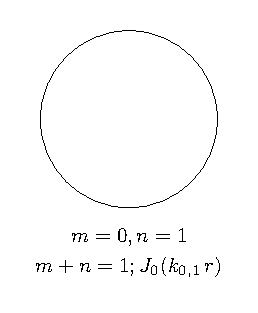
\includegraphics[scale=1]{Figuras/Modos_Vibracion_Membrana_0_1.tex}
\end{figure}
\end{frame}
\begin{frame}
\frametitle{Modo $m=0, n=2$}
\begin{figure}
    \centering
    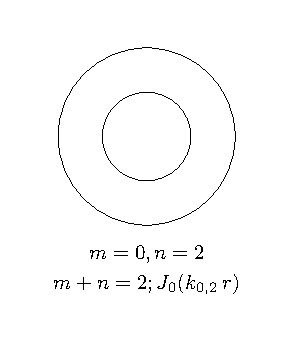
\includegraphics[scale=1]{Figuras/Modos_Vibracion_Membrana_0_2.tex}
\end{figure}
\end{frame}
\begin{frame}
\frametitle{Modo $m=0, n=3$}
\begin{figure}
    \centering
    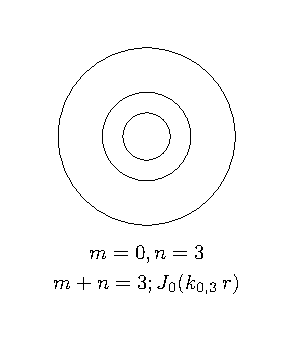
\includegraphics[scale=1]{Figuras/Modos_Vibracion_Membrana_0_3.tex}
\end{figure}
\end{frame}
\begin{frame}
\frametitle{Modos de vibración degenerados}
Las degeneraciones de orden 2 para $m > 0$ surgen de nuevo debido a los 2 grados espaciales de libertad ($x$ e $y$, $r$ y $\varphi$).
\\
\bigskip
\pause
La simetría rotacional de la membrana circular: es invariante en rotaciones arbitrarias.
\end{frame}
\begin{frame}
\frametitle{Modo $m=1, n=1$}
\begin{figure}
    \centering
    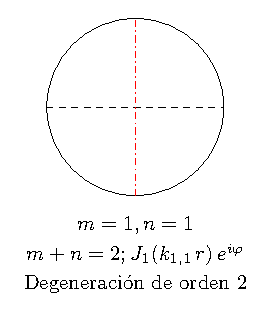
\includegraphics[scale=1]{Figuras/Modos_Vibracion_Membrana_1_1.tex}
\end{figure}
\end{frame}
\begin{frame}
\frametitle{Modo $m=1, n=2$}
\begin{figure}
    \centering
    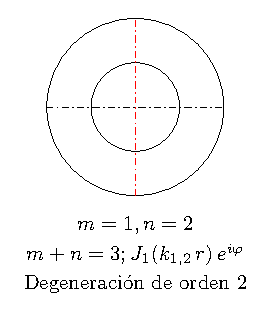
\includegraphics[scale=1]{Figuras/Modos_Vibracion_Membrana_1_2.tex}
\end{figure}
\end{frame}
\begin{frame}
\frametitle{Modo $m=1, n=3$}
\begin{figure}
    \centering
    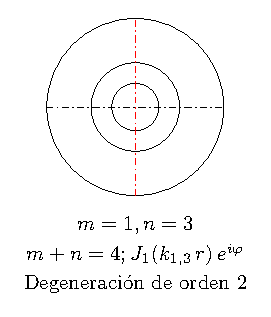
\includegraphics[scale=1]{Figuras/Modos_Vibracion_Membrana_1_3.tex}
\end{figure}
\end{frame}
\begin{frame}
\frametitle{Modo $m=2, n=1$}
\begin{figure}
\centering
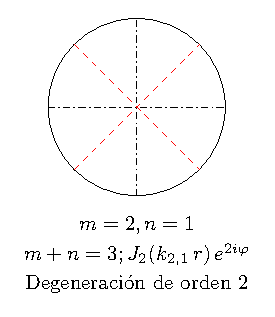
\includegraphics[scale=1]{Figuras/Modos_Vibracion_Membrana_2_1.tex}
\end{figure}
\end{frame}
\begin{frame}
\frametitle{Modo $m=2, n=2$}
\begin{figure}
    \centering
    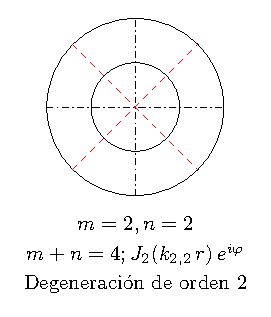
\includegraphics[scale=1]{Figuras/Modos_Vibracion_Membrana_2_2.tex}
\end{figure}
\end{frame}
\begin{frame}
\frametitle{Modo $m=2, n=3$}
\begin{figure}
    \centering
    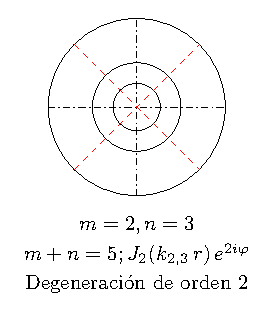
\includegraphics[scale=1]{Figuras/Modos_Vibracion_Membrana_2_3.tex}
\end{figure}
\end{frame}
\begin{frame}
\frametitle{Extendiendo el estudio}
Una siguiente parte de estudio sobre los modos de vibración de una membrana circular, es sobre la manera de visualizar las oscilaciones.
\\
\bigskip
\pause
En las figura anteriores, se nota la descripción por zonas en la membrana, para extender el estudio, es ahora necesario el apoyo de herramientas ya sea de programación o de software matemático.
\end{frame}
\begin{frame}
\frametitle{Extendiendo el estudio}
En la siguiente figura se presenta el mismo arreglo descriptivo, pero ahora con más información, se utilizó el software \texttt{Mathematica}, para resolver la ecuación diferencial, obtener los ceros de las funciones de Bessel y finalmente, ocupar una rutina de graficación para visualizar de otra manera el mismo resultado:
\end{frame}
\begin{frame}
\frametitle{Otra visualización}
\begin{figure}
    \centering
    \includegraphics<-2>[scale=0.72]{Imagenes/Vibracion_Membrana_01.eps}
\end{figure}
\end{frame}
\begin{frame}
\frametitle{Otra visualización}
\begin{figure}
    \centering
    \includegraphics<-2>[scale=0.72]{Imagenes/Vibracion_Membrana_02.eps}
\end{figure}
\end{frame}
\begin{frame}
\frametitle{Otra visualización}
\begin{figure}
    \centering
    \includegraphics<-2>[scale=0.72]{Imagenes/Vibracion_Membrana_03.eps}
\end{figure}
\end{frame}
\begin{frame}
\frametitle{Animación}
Es posible realizar una animación de las gráficas obtenidas, en el ejemplo: $m=0$ y $n=1$.
\end{frame}

\end{document}